%=========================================================================
% sec-results
%=========================================================================


\section{Results}
\label{sec-results}

%=========================================================================
% fig-results-tbb-omp.tex
%=========================================================================

\begin{figure}[!hbt]

  \centering
  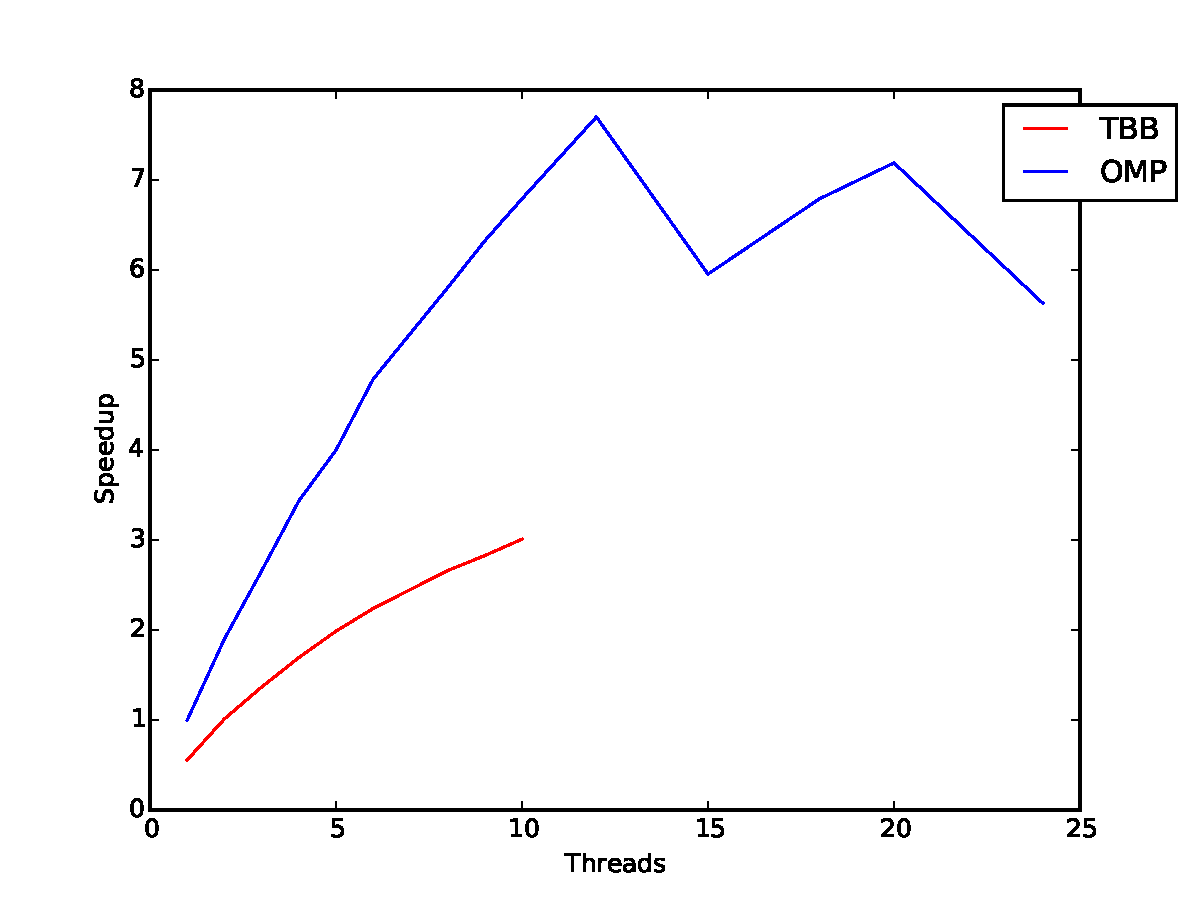
\includegraphics[width=0.5\tw]{fig-results-tbb-omp.pdf}

  \caption{\textbf{Strong scaling of OMP and TBB without vectorization --} Strong scaling results for a minibatch size of 360 for OMP and TBB without vectorization. The original author's code (TBB) does not work for more than 10 threads and thus results are not shown for TBB with >10 threads. Note the dip when OMP goes beyond 12 threads which is a result of increased communication cost across 2 chips.}

  \label{fig-results-tbb-omp}

  \centering
  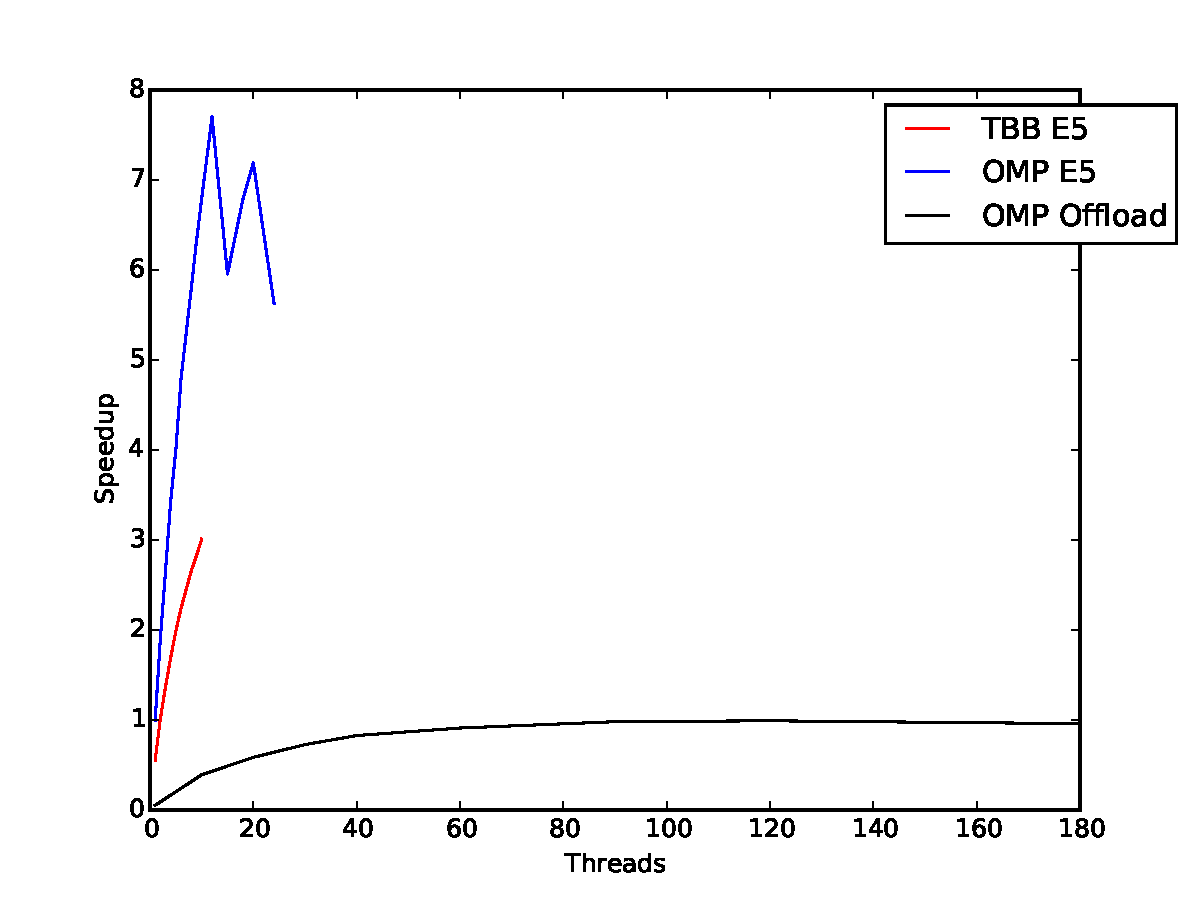
\includegraphics[width=0.5\tw]{fig-results-mic.pdf}

  \caption{\textbf{Strong scaling of offloaded MIC without vectorization --} Strong scaling results for offloaded MIC code as compared to TBB and OMP on the compute node. The offloaded MIC code performs poorly, likely due to too much serial work or lack of vectorization.}

  \label{fig-results-mic}

\end{figure}

% %=========================================================================
% fig-results-mic.tex
%=========================================================================

\begin{figure}[!hbt]

  \centering
  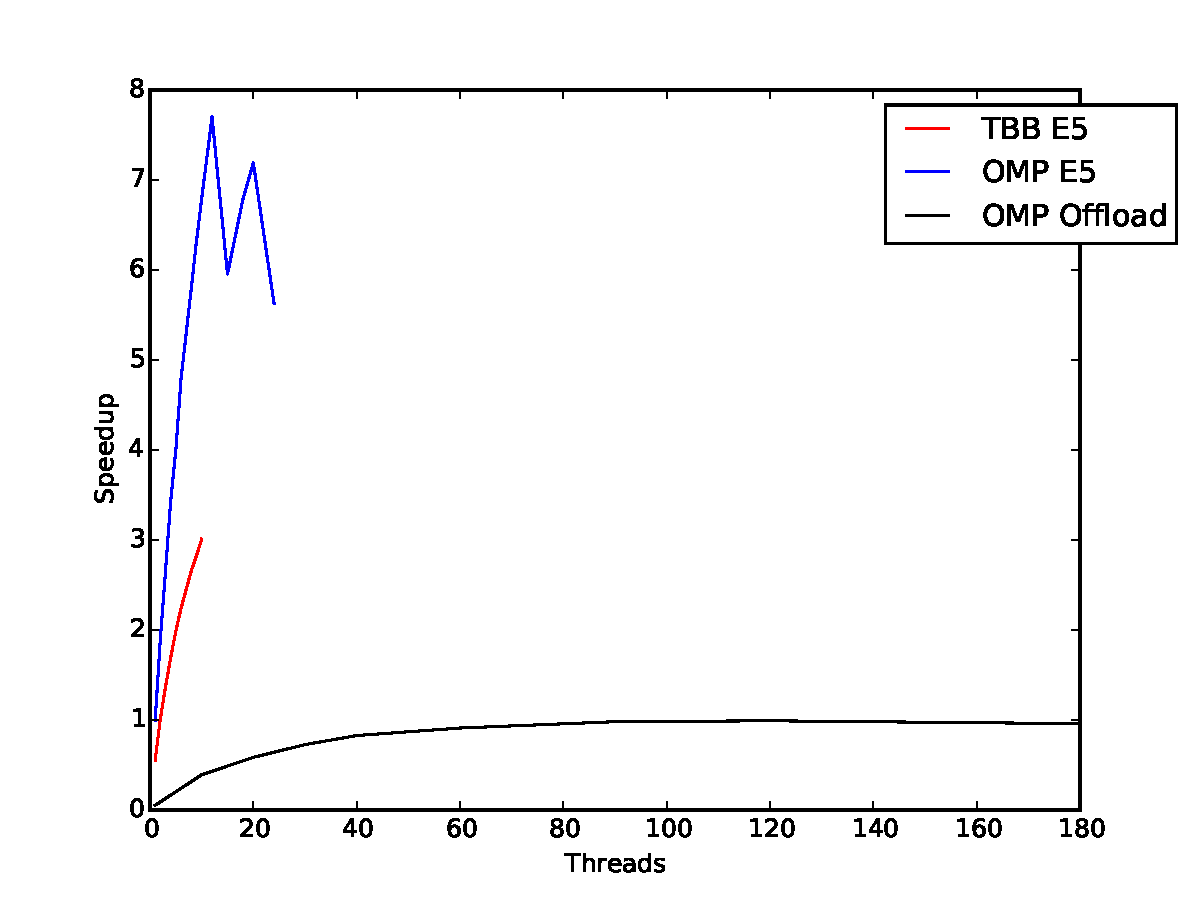
\includegraphics[width=0.5\tw]{fig-results-mic.pdf}

  \caption{\textbf{Strong scaling of OMP and TBB without vectorization --} Strong scaling results for a minibatch size of 360 for OMP and TBB without vectorization. The original author's code (TBB) does not work for more than 10 threads and thus results are not shown for TBB with >10 threads. Note the dip when OMP goes beyond 12 threads which is a result of increased communication cost across 2 chips.}

  \label{fig-results-mic}

\end{figure}


To understand how our improvements to the Tiny CNN implementation perform we tested various versions of implementation on a relatively simple neural network which was 6-layers deep and used average pooling, hyperbolic tangent as the activation function, RMSProp for gradient descent, and mean-squared error as our loss function.

 timed training this network for the MNIST dataset (handwritten digit recognition) with a minibatch size of 360 for a single epoch. We do not report our accuracy results for the dataset as they are all the same and are in line with standard accuracies for this dataset.

\subsection{TBB vs. OMP without AVX}
\label{sec-results-tbb-vs-omp}


To analyze how well our parallelized CNN with OMP compared to the original implementation which used TBB we ran a strong scaling study for both, with a minibatch size of 360. The results in Figure~\ref{fig-results-tbb-omp} show that the OMP implementation gets much larger speedup as threads increase from 1 to 10.

We believe that our OMP version outperformed TBB by being doing \textit{less} parallelization than the original TBB code. The original TBB code used parallelization at many levels, including at the lowest for-loop level. This likely results in significant synchronization and thread-handling time which outstrips potential gains made by parallelizing low-work for-loops. Instead, by implementing our OMP parallelization at the minibatch level we distributed significant work to each thread such that synchronization and thread creation did not become a bottleneck.

\subsection{MIC Offloading without AVX}
\label{sec-results-mic}

%=========================================================================
% fig-result-tbb-omp-avx.tex
%=========================================================================

\begin{figure}[!hbt]

  \centering
  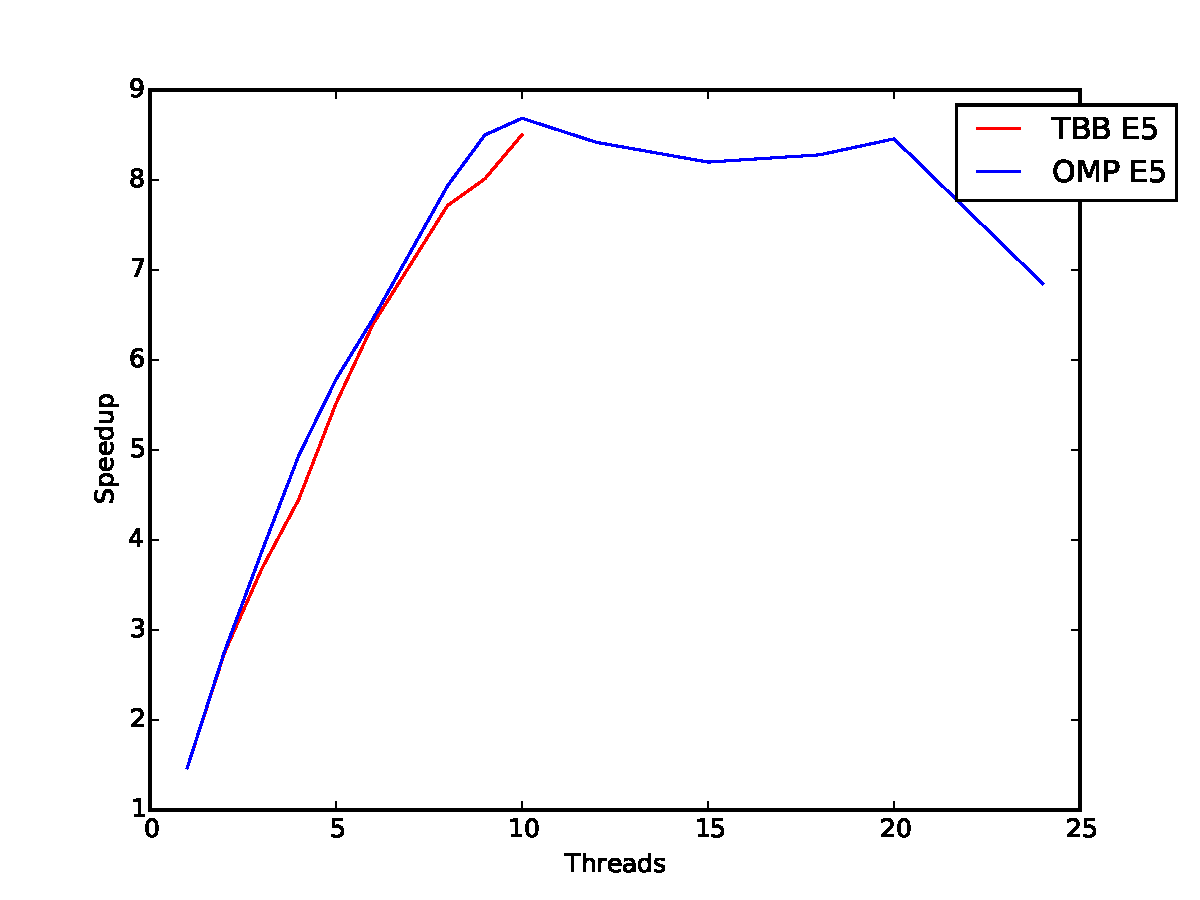
\includegraphics[width=0.5\tw]{fig-results-tbb-omp-avx.pdf}

  \caption{\textbf{Strong scaling of OMP and TBB with vectorization --} Strong scaling results for a minibatch size of 360 for OMP and TBB with explicit vectorization. TBB performs much more similarly to OMP as compared to without vectorization.}

  \label{fig-results-tbb-omp-avx}

  \centering
  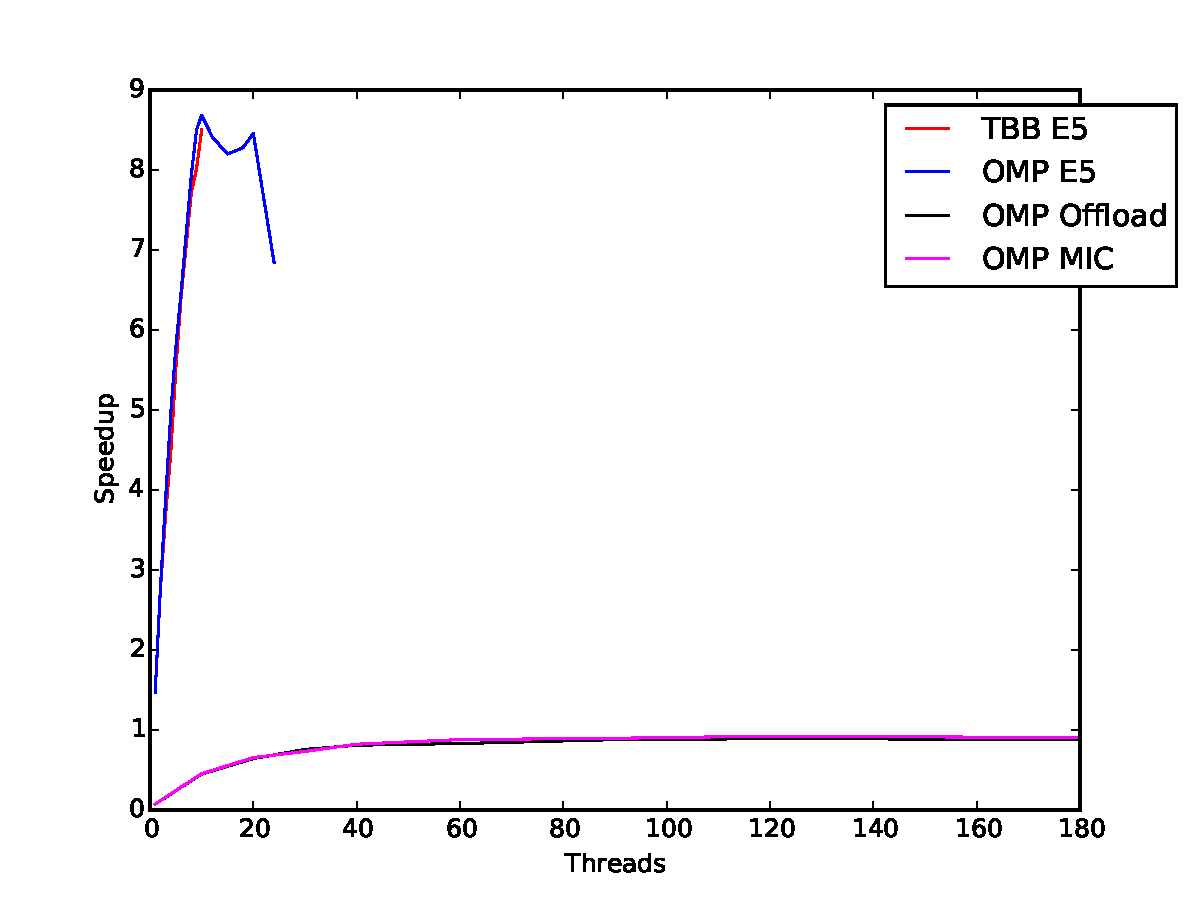
\includegraphics[width=0.5\tw]{fig-results-mic-avx.pdf}

  \caption{\textbf{Strong scaling of MIC with AVX512 --} Strong scaling comparison of offloaded MIC code (OMP Offloaded), direct MIC code (OMP MIC), and OMP/TBB on the compute nodes. All code used explicit vectorization. Offloaded and Direct MIC code perform similarly, but both perform worse than without AVX512 vectorization.}

  \label{fig-results-mic-avx}

\end{figure}

% %=========================================================================
% fig-results-mic-avx.tex
%=========================================================================

\begin{figure}[!hbt]

  \centering
  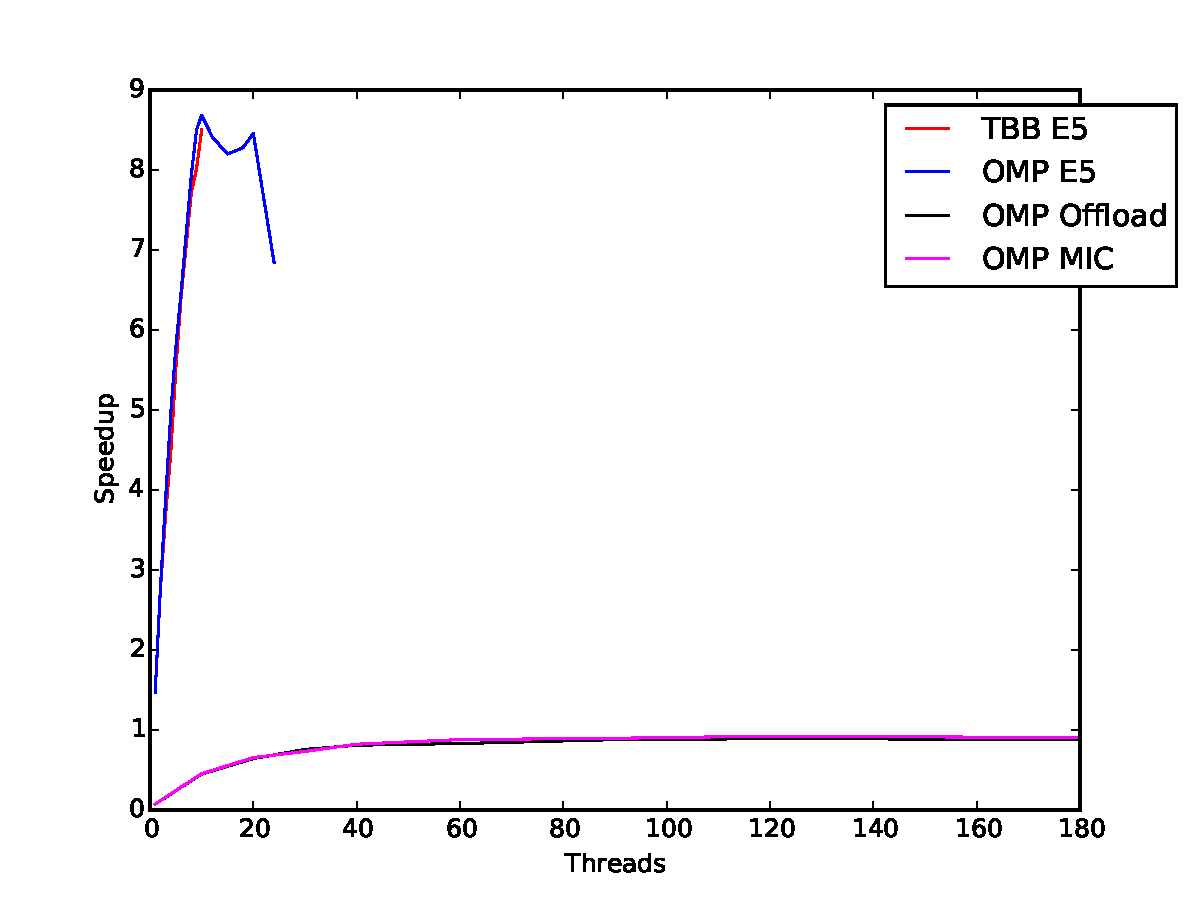
\includegraphics[width=0.5\tw]{fig-results-mic-avx.pdf}

  \caption{\textbf{Strong scaling of MIC with AVX512 --} Strong scaling comparison of offloaded MIC code (OMP Offloaded), direct MIC code (OMP MIC), and OMP/TBB on the compute nodes. All code used explicit vectorization.}

  \label{fig-results-mic-avx}

\end{figure}


To see how well offloaded OMP code performed we did the same strong scaling study as in section~\ref{sec-results-tbb-vs-omp}. The results in Figure~\ref{fig-results-mic} show that the offloaded code performs much worse than code run directly on the main compute nodes, regardless of thread count. However, we do see speedup increase as thread count increases, but even with 180 threads the offloaded MIC code is not as fast as single threaded code on the compute node.

We suspect that the reasons for poor performance are two-fold. First, the serial work required per batch is enough to outweight potentialy benefits gained by doing the parallel work quickly. Second, without vectorization--and there is no vectorization done by the compiler--the Co-processors simply suffer too much due to the poor computation power each core has.

\subsection{TBB vs. OMP with AVX}
\label{sec-results-tbb-omp-avx}

After implementing manual vectorization, tuning and memory layout improvements in theory both the TBB and OMP versions of our CNN should see larger speedups than before. In figure~\ref{fig-results-tbb-omp-avx} we see that this is indeed the case. We see TBB do drastically better, with speedups very close to that of our OMP implementation. Further, we see our OMP implementation increase its peek speedup to about 8.75 where as in figure~\ref{fig-results-tbb-omp} its peak speedup was approximately 7.75.

The reason why we see larger speedups for TBB is because TBB already was slower, and thus could get more significant improvements from explicit use of AVX intrinsics. Further TBB flexibly chooses when to use threads, and may choose to use fewer threads at a lower level when loops are being vectorized. OMP sees smaller gains because it was already fast on these low-level for-loops because of a lack of synchronization and thread-handling overhead. However we still see increased speedup for OMP because computations are still reduced overall.

\subsection{MIC with AVX}
\label{sec-results-mic-avx}

For our final results we compared the performance of our offloaded MIC code and direct MIC code (run directly on the MIC) when using AVX512 vectorization. The strong scaling results of doing so are shown in figure~\ref{fig-results-mic-avx}.

Surprisingly when we implement AVX512 for the MICs our code actually saw smaller speedups than before. This is surprising as one would normally expect vectorization to improve speed. However, vectorization comes with its own overheads and when dealing with small images to begin with (32x32) in the MNIST dataset which get smaller as the images pass through the layers there is not much room for vectorization. This is because AVX512 supports 8 doubles in a vector register, and when consider edge cases of each layer, means only 1 or 2 vector instructions fit per dimension per layer. This means that vectorization which comes with complication overheads is simply not worth it and slows our code down even further.

We suspect that we would see better speedup if larger images were used (256x256) for instance, but were unable to obtain a dataset with larger images for testing.
